\section{Experimento 1: Red de Starbucks}

\subsection{Descripción del contexto}

El experimento fue realizado en una red de FibertelZone, por medio de una conexión Wi-Fi en un local de Starbucks de Corrientes y Malabia. Dentro de la red se encuentran conectadas aproximadamente 10 notebooks y muchos celulares, además del router. La fecha de captura es Domingo 9 de Octubre de 2017.

\subsection{Descripción de la captura}

Capturamos 12000 paquetes. 

%% distribucion de protocolos (grafico)
\begin{figure}[H]
\centering
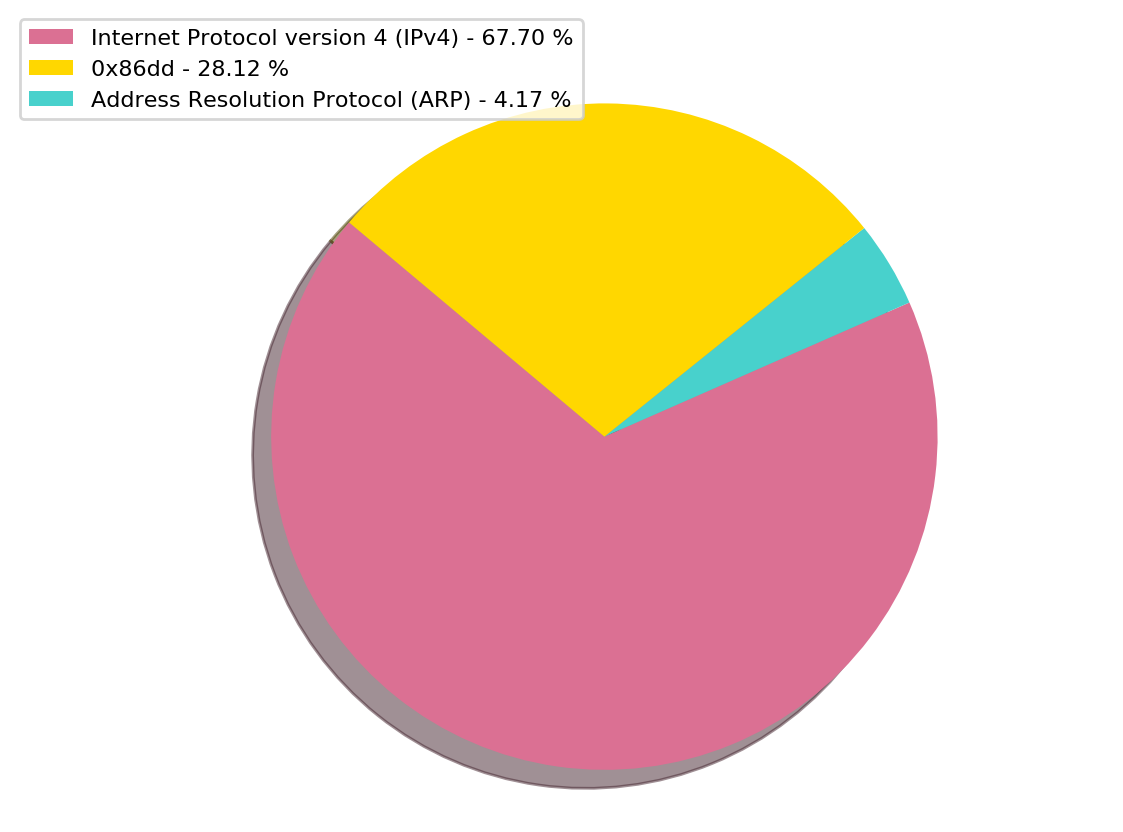
\includegraphics[width=0.7\textwidth]{protocolosRed1.png}
\caption{Gráfico que muestra la distribución de protocolos en la red.}
\label{broadcast2}
\end{figure}

%% grafico de broadcast
\begin{figure}[H]
\centering
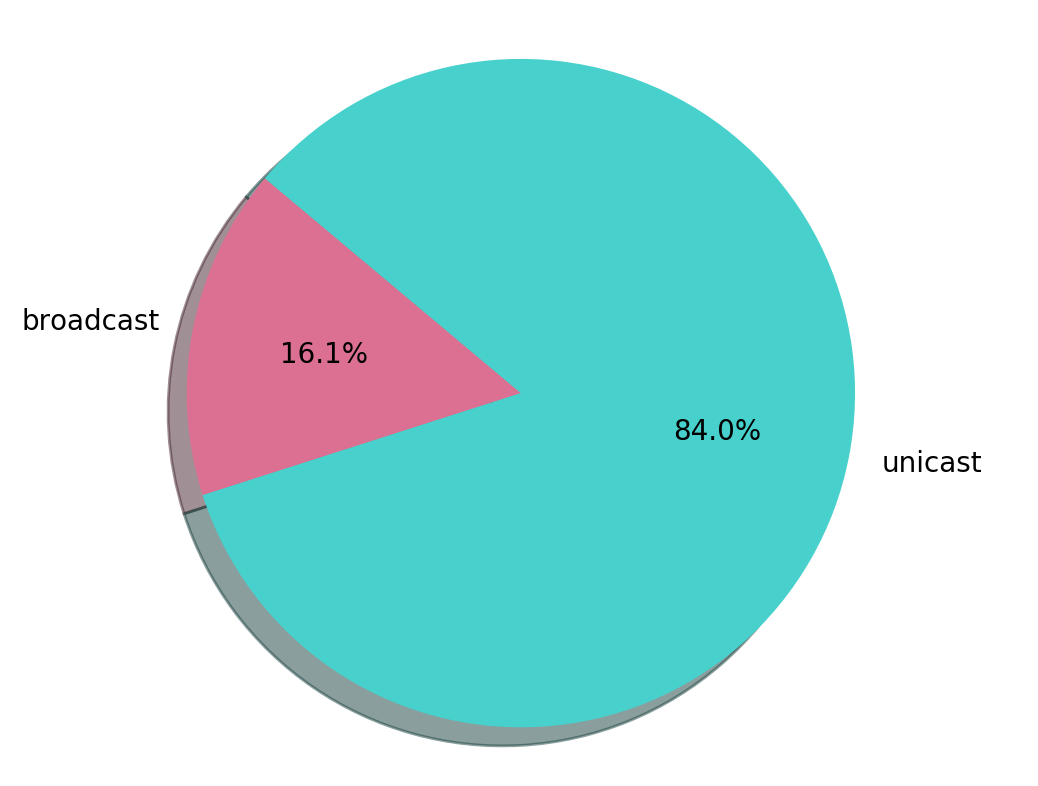
\includegraphics[width=0.7\textwidth]{broadcastRed1.png}
\caption{Gráfico que muestra los porcentajes de tráfico broadcast y unicast.}
\label{broadcast1}
\end{figure}

\subsection{Análisis de la captura}

%% grafico entropia S1
\begin{figure}[H]
\centering
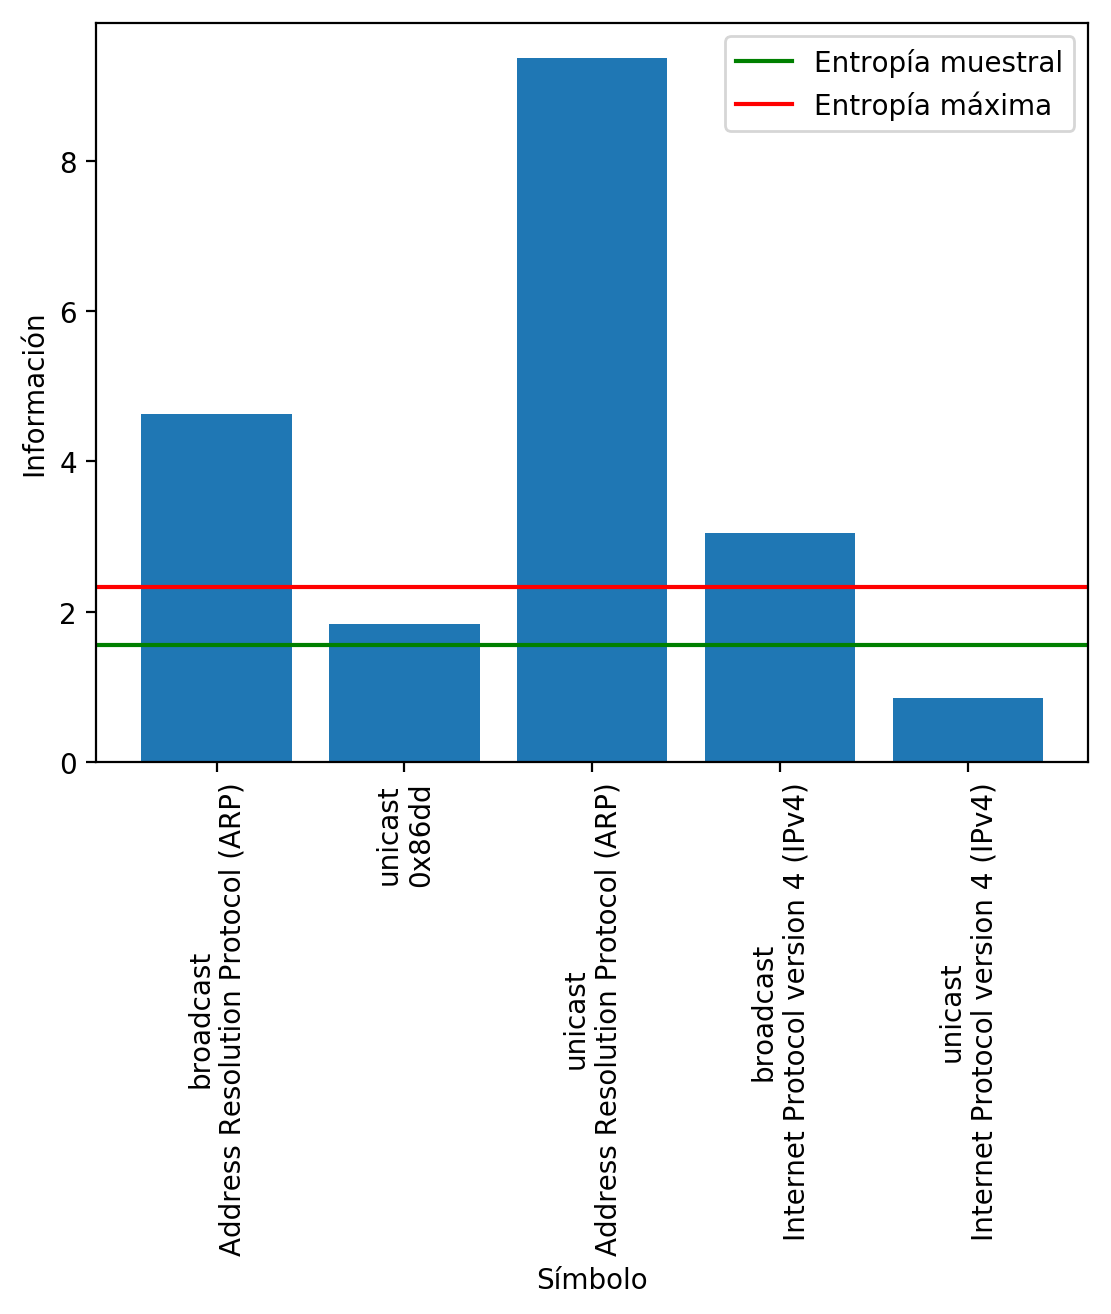
\includegraphics[width=0.7\textwidth]{entropiaS1Red1.png}
\caption{Gráfico de la información de los símbolos de la fuente $S_1$ observados en esta red. Se muestra la entropía muestral de $S_1$ y su entropía máxima.}
\label{entropias1_2}
\end{figure}

%% grafico entropia S2
\begin{figure}[H]
\centering
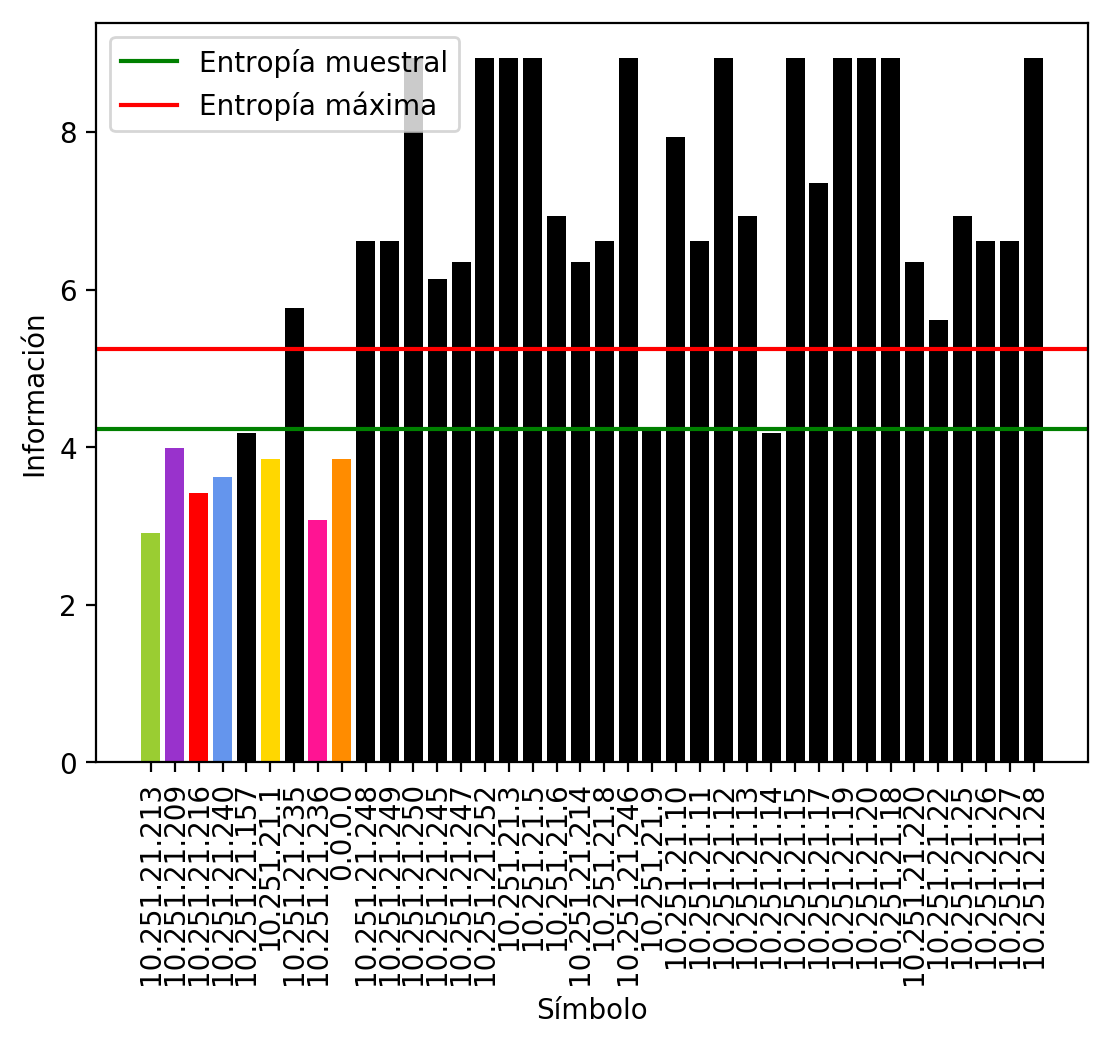
\includegraphics[width=0.7\textwidth]{entropiaS2Red1.png}
\caption{Gráfico de la información de los símbolos de la fuente $S_2$ observados en esta red. Se muestra la entropía muestral de $S_2$ y su entropía máxima.}
\label{entropias2_2}
\end{figure}

%% red ARP
\begin{figure}[H]
\centering
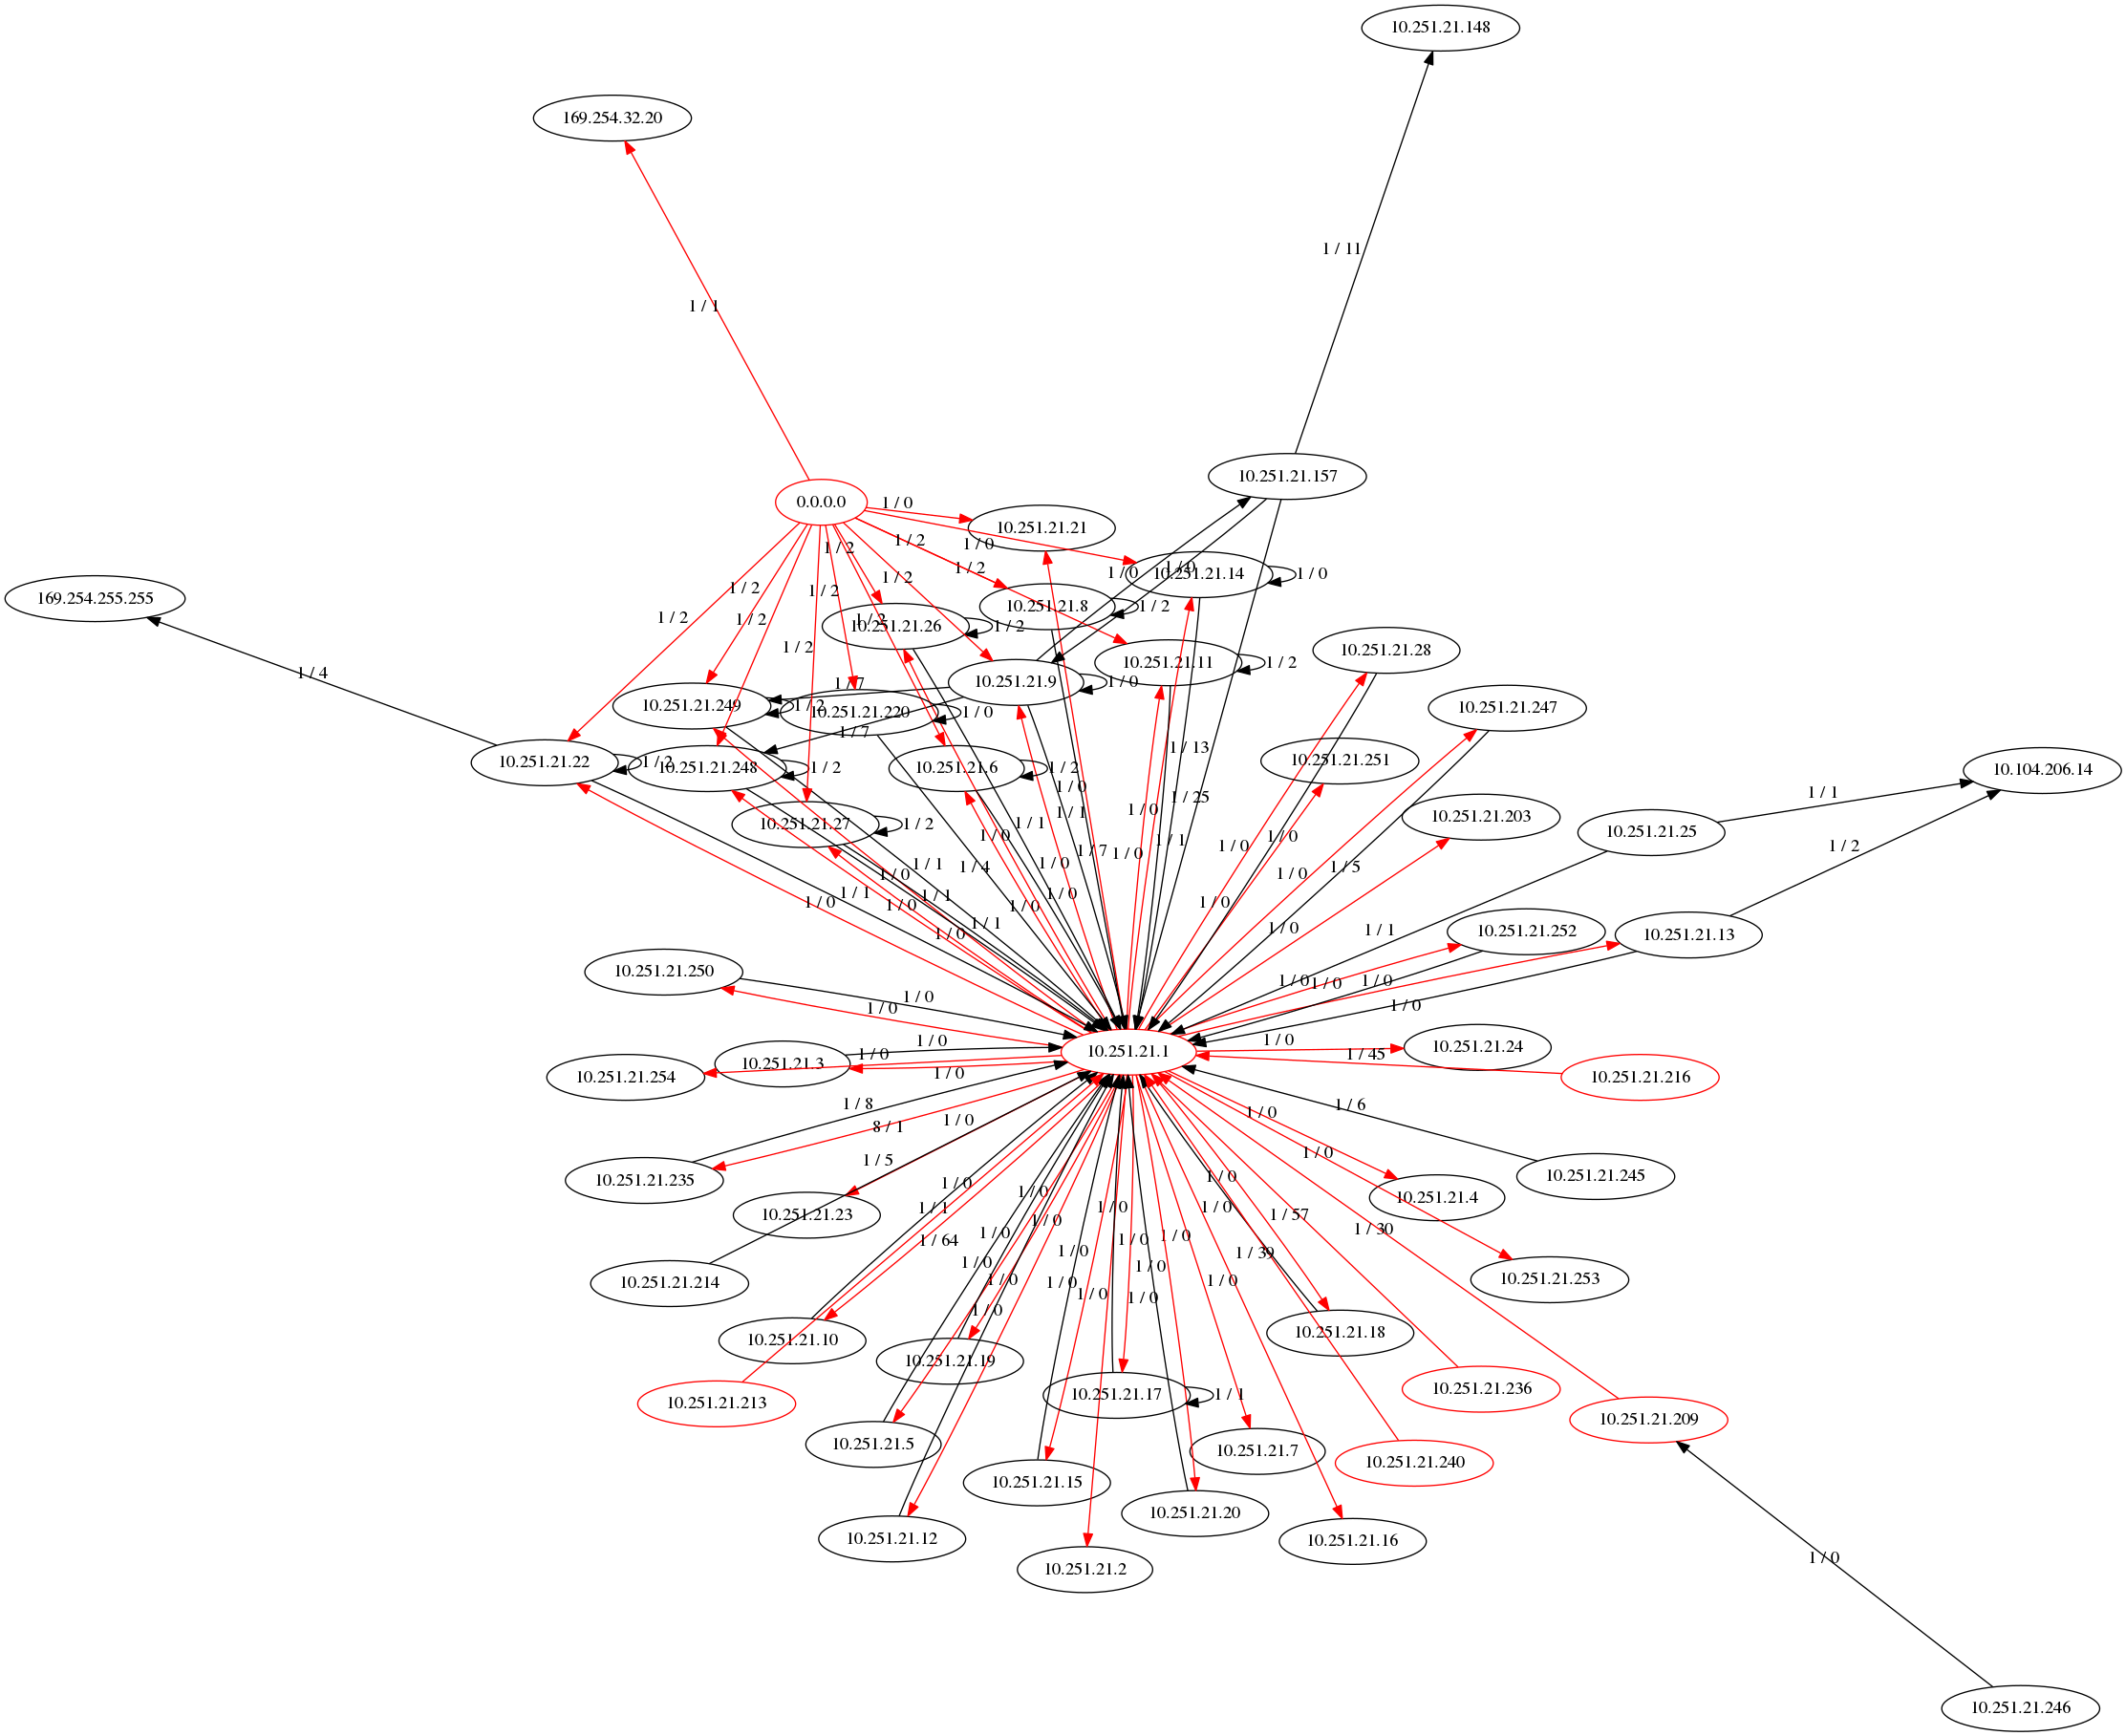
\includegraphics[width=\textwidth]{grafoRed1.png}
\caption{Grafo de la red de mensajes ARP subyacente.}
\label{grafo1}
\end{figure}
